\chapter{Results and Evaluation}
\label{chapter:results-and-evaluation}

This chapter will focus on the data obtained in the project. For clarity, there is a separate section on each fractal, as they are quite different and had their own sets of representative views. A small explanation of the expected results will be given for each fractal. For the temporal caching, there were some tests that could be performed, that could not be performed with the signed distance field, because they involved animations that either changed the geometry or travelled far outside acceptable range for the signed distance field. Therefore, static image tests will be separated from animation tests. After each set of results is presented, discussion and evaluation of those results will be done.\newline

The unoptimized time given is the time taken to execute the entire geometry render pass, in nanoseconds. The performance gain (or loss) is measured by obtaining the percentage difference between the unoptimized method, and the optimized one, with this equation:

\begin{equation}
	diff = \frac{unopt - opt}{unopt} * 100
\end{equation}

where unopt and opt are the unoptimized time and optimized time, respectively.

\section{Mandelbulb Static Image Tests}

\subsection{Representative Views}

\begin{figure}[ht]
	\centering

	\begin{subfigure}[c]{0.45\linewidth}
		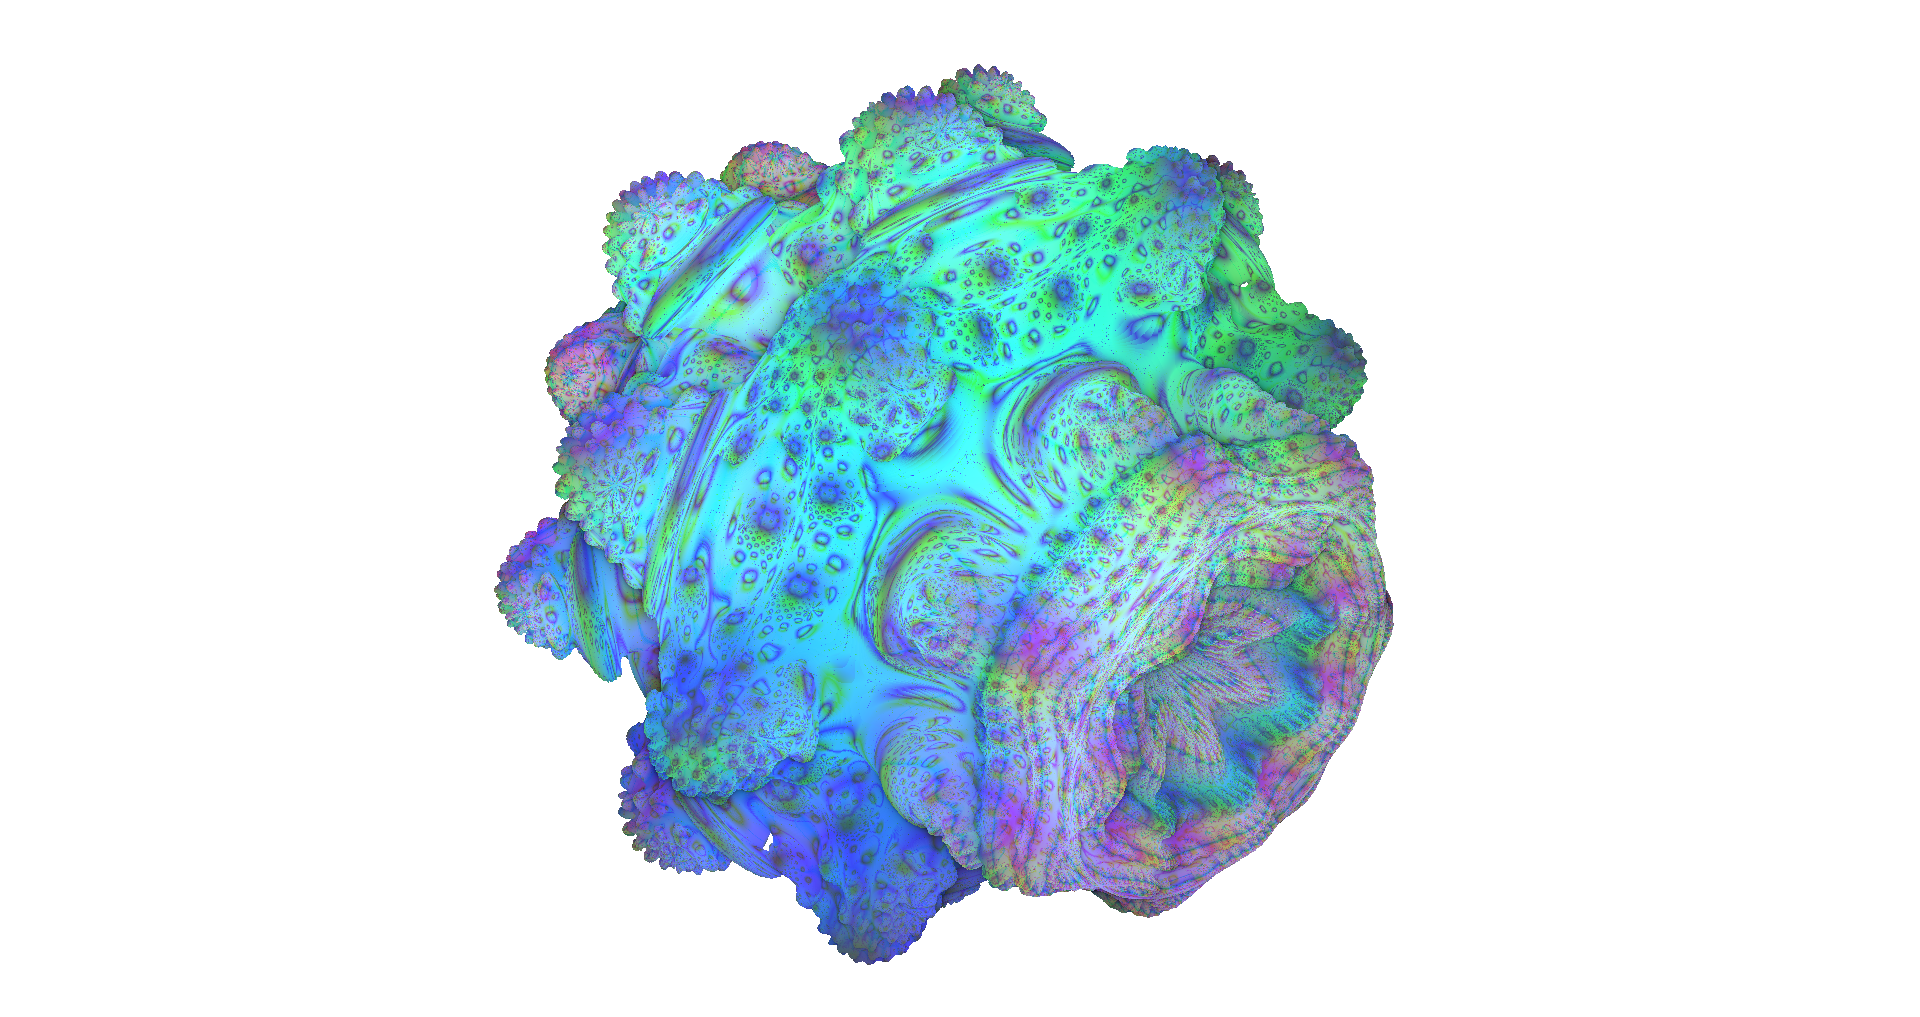
\includegraphics[width=\linewidth, frame]{Images/Results/Mandelbulb-View-01-Default}
		\caption{Mandelbulb: Default View.}
		\label{figure:mandelbulb-view-01-default}
	\end{subfigure}
	\hfill
	\begin{subfigure}[c]{0.45\linewidth}
		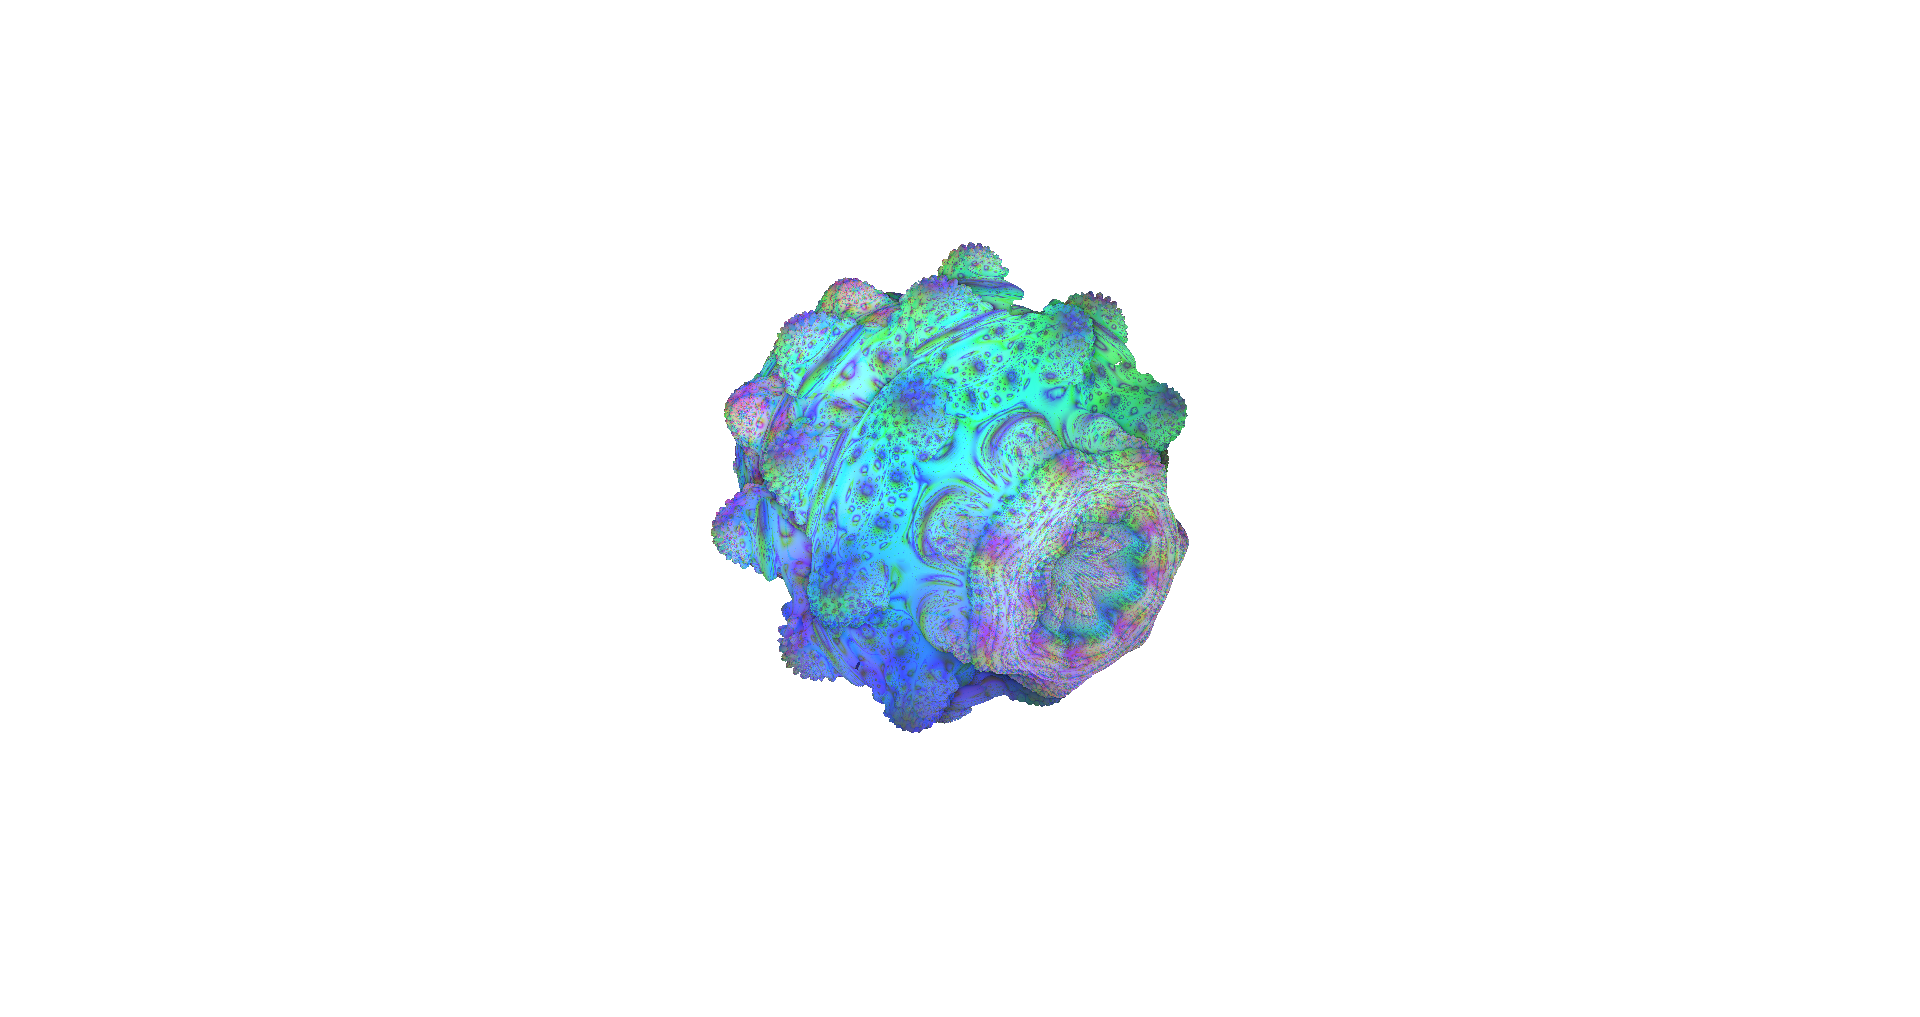
\includegraphics[width=\linewidth, frame]{Images/Results/Mandelbulb-View-02-Empty-Space}
		\caption{Mandelbulb: Zoomed Out View.}
		\label{figure:mandelbulb-view-02-empty-space}
	\end{subfigure}
	\hfill
	\begin{subfigure}[c]{0.45\linewidth}
		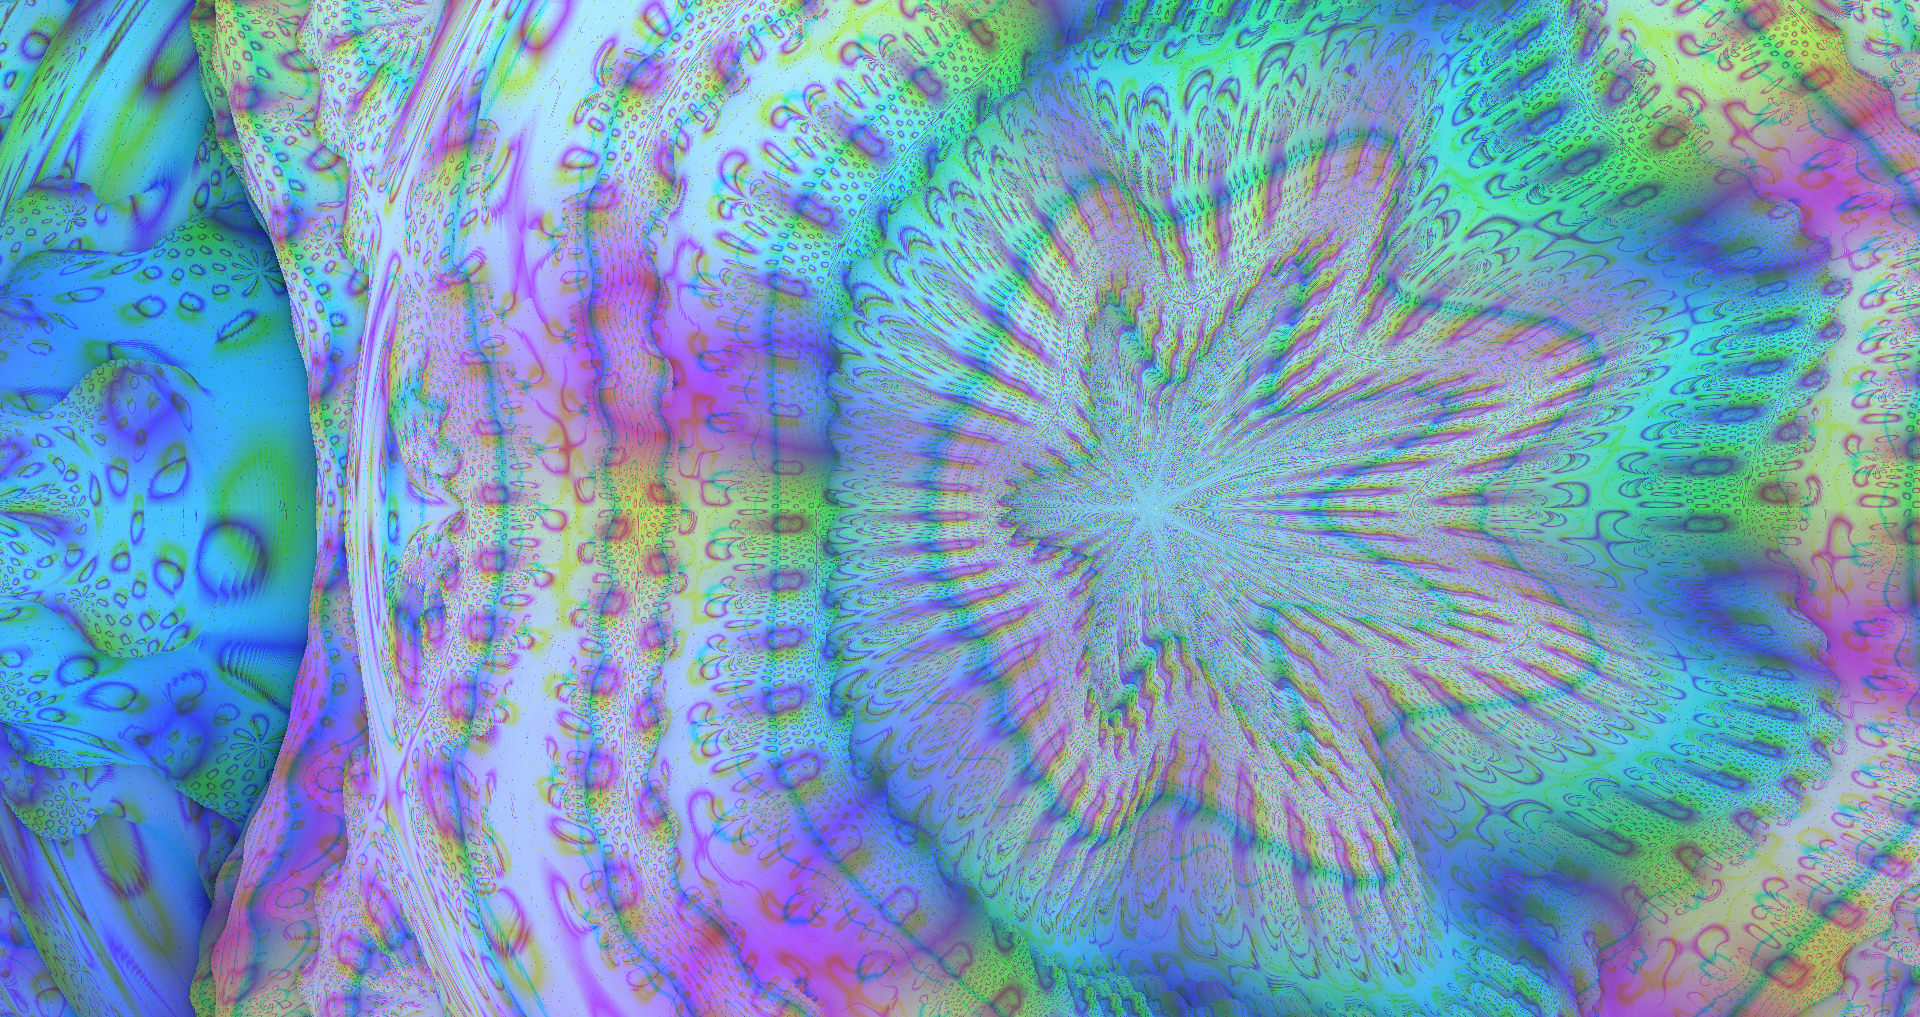
\includegraphics[width=\linewidth, frame]{Images/Results/Mandelbulb-View-03-No-Space}
		\caption{Mandelbulb: Zoomed In View.}
		\label{figure:mandelbulb-view-03-no-space}
	\end{subfigure}
	\hfill
	\begin{subfigure}[c]{0.45\linewidth}
		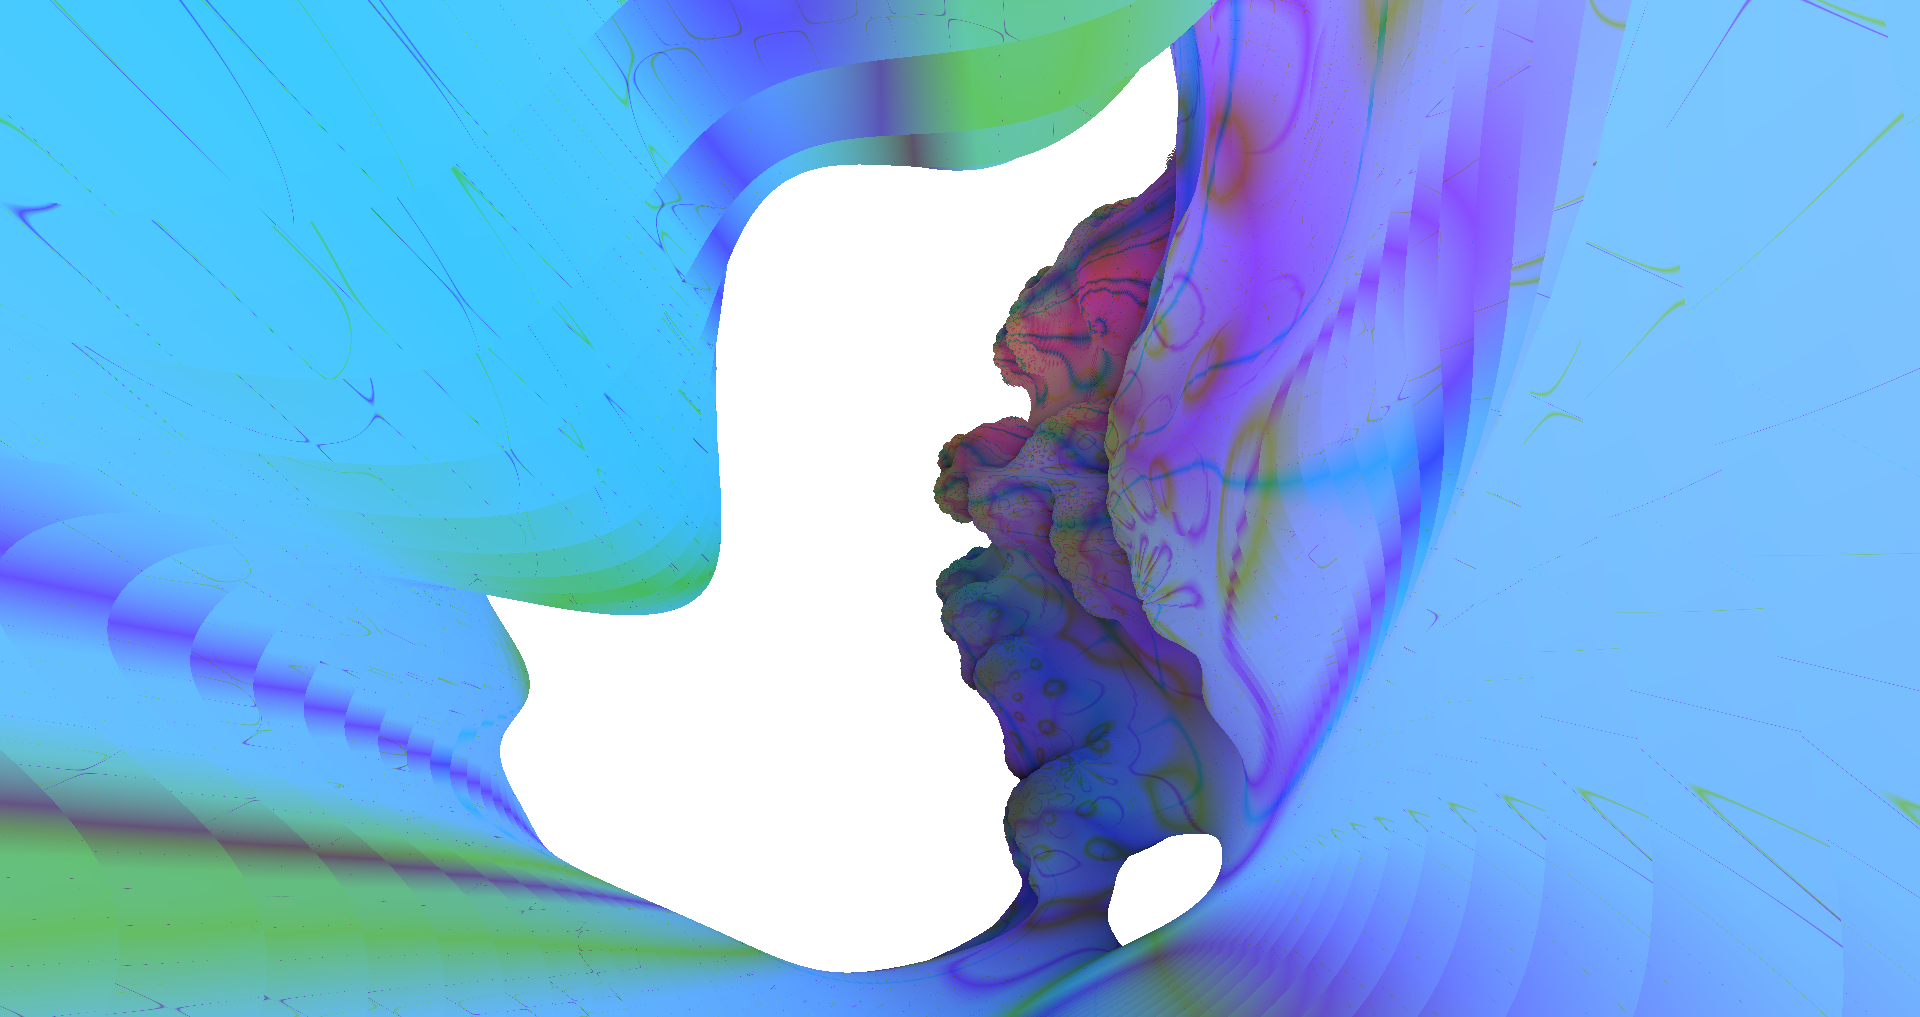
\includegraphics[width=\linewidth, frame]{Images/Results/Mandelbulb-View-04-Bottleneck}
		\caption{Mandelbulb: Bottleneck View.}
		\label{figure:mandelbulb-view-04-bottleneck}
	\end{subfigure}

	\caption{Four representative views of the Mandelbulb fractal, used in performance tests.}
	\label{figure:mandelbulb-views}
\end{figure}

Figure \ref{figure:mandelbulb-views} shows the four representative views used for performance measurements. Figure \ref{figure:mandelbulb-view-01-default} shows the default view, which is not expected to be particularly well suited to any performance measurement, to get a general-case overview of the performance differences between the methods used. Figure \ref{figure:mandelbulb-view-02-empty-space} is the view intended to include the most empty space (short of simply turning around and not looking at the fractal at all), and by contrast figure \ref{figure:mandelbulb-view-03-no-space} is intended to include the least. Lastly, figure \ref{figure:mandelbulb-view-04-bottleneck} includes a mix of depth and smoothness, and some bottlenecks.

\subsection{Expected Results}

The view of the Mandelbulb fractal involves quite a bit of empty space, unlike the Hall of Pillars fractal, which contains none. The expected result is that the Temporal caching method will give a slight performance boost to views with empty space, especially around the edges of the fractal, where more iterations would normally occur, but huge boosts are not expected since the Mandelbulb does not contain so many bottlenecks, and the depth variance is small. For still images, though, the temporal caching should give a boost no matter what is being looked at, as long as the camera does not move.\newline

For the signed distance field, it entirely depends on whether searching through the three-dimensional grid is less expensive than calculating the signed distance function or not, as the signed distance field is intended to provide a cheaper alternative every iteration, not to reduce the number of iterations as the temporal caching is supposed to do. The prediction is that the more costly the function, the more benefit will be seen, but that, since the Mandelbulb function is relatively cheap, there won't be much benefit, if any, with the distance function used here.

\subsection{Results}

Table \ref{table:mandelbulb-static-results} shows the results obtained for the four representative views of the Mandelbulb fractal. SDF stands for signed distance field, and TC stands for temporal caching.

\begin{table}[ht]
	\centering
	\begin{tabular}{||p{0.2\linewidth}|p{0.29\linewidth}|p{0.23\linewidth}|p{0.23\linewidth}||}
		\hline
		View & Unoptimized Time (ns) & SDF Difference (\%) & TC Difference (\%)\\
		\hline\hline
		Default & 1272832 & -152.40 & 22.26\\
		\hline
		Zoomed Out &1083328  & -196.82 & 8.67\\
		\hline
		Zoomed In & 1241088 & -33.81 & -2.30\\
		\hline
		Bottleneck & 1593888 & -6.94 & 7.01\\
		\hline
	\end{tabular}
	\caption{A table showing the performance differences between the two optimization methods and the base, unoptimized rendering, for four different views of the Mandelbulb.}
	\label{table:mandelbulb-static-results}
\end{table}

\subsection{Evaluation}

\subsubsection{Signed Distance Field}

Clearly, the signed distance field did not do well for this fractal. The biggest negative difference was for the zoomed out view. This may be because most of the rays would have been destined to fall outside of the boundary of the field, so they would have fallen back on the regular signed distance field

\section{Mandelbulb Animation Tests}

\subsection{Animations}

\subsection{Expected Results}

\subsection{Results}

\subsection{Evaluation}

\section{Hall of Pillars Static Image Tests}

\subsection{Representative Views}

\subsection{Expected Results}

This fractal contains many bottlenecks (the ray has to pass close to lots of geometry before reaching any surface), so the temporal caching method is expected to perform better here than with the Mandelbulb, in terms of performance difference. A view with very simple geometry was also chosen because of this, as the prediction is that the temporal caching method will provide minimal benefit where these bottlenecks don't exist, the surface is very smooth, or the distance to the surface is very small.\newline

The signed distance field was very tricky to test, since the fractal does not fit neatly into a small box, like the Mandelbulb. Because of this, during tests for the signed distance field, a ray culling step was added. Any ray not destined to intersect with the main signed distance field area is not followed. This gives a sort of cross-section of the fractal, and this was what was used. This step was added to all tests to be compared with the test for the signed distance field, for consistency. The signed distance field is not expected to give a huge benefit here, as the relative expense of the distance estimator is not very high.

\subsection{Results}

\begin{table}[ht]
	\centering
	\begin{tabular}{||p{0.2\linewidth}|p{0.29\linewidth}|p{0.23\linewidth}|p{0.23\linewidth}||}
		\hline
		View & Unoptimized Time (ns) & SDF Difference (\%) & TC Difference (\%)\\
		\hline\hline
		Default &  &  & \\
		\hline
		Zoomed Out &  &  & \\
		\hline
		Zoomed In &  &  & \\
		\hline
		Bottleneck &  &  & \\
		\hline
	\end{tabular}
	\caption{A table showing the performance differences between the two optimization methods and the base, unoptimized rendering, for five different views of the Hall of Pillars fractal.}
	\label{table:hall-of-pillars-static-results}
\end{table}

\subsection{Evaluation}

\section{Hall of Pillars Animation Tests}

\subsection{Animations}

\subsection{Expected Results}

\subsection{Results}

\subsection{Evaluation}